% ==============================================
% !TEX root = ./critics.tex
% ==============================================
% ==============================================
\section{Motivating Examples and Tool Features}
\label{sec:motivation}
% ==============================================
%\begin{figure*}
%\centering
%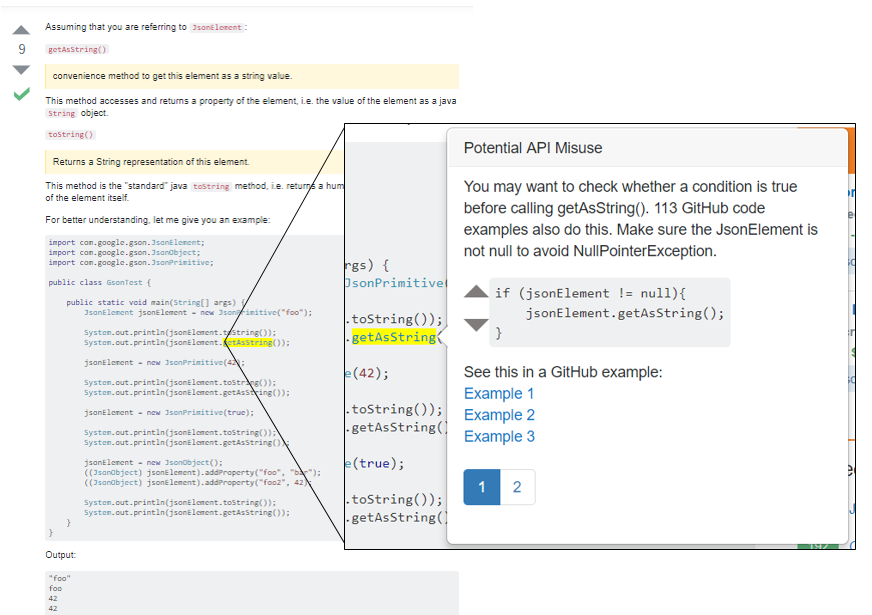
\includegraphics[width=0.6\textwidth]{json_ex1_context.PNG}
%  \vspace{.1in}
%  \caption{A code snippet that does not properly check {\tt JsonElement.getAsString}.\protect\footnotemark}
%  \label{fig:so_example}
%\end{figure*}
%
%\begin{figure*}[t!]
%\centering
%  \begin{subfigure}[t]{0.48\textwidth}
%  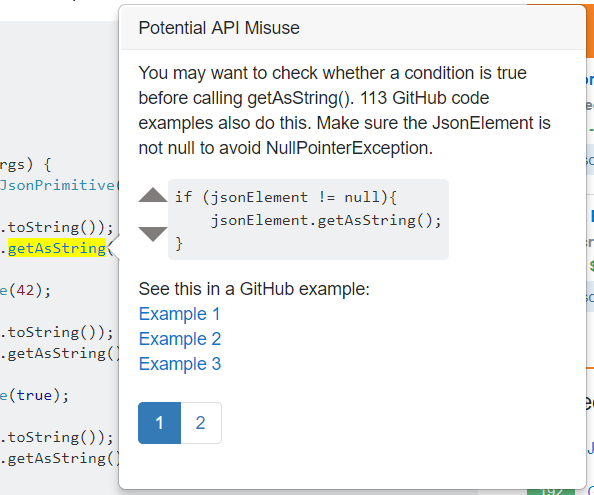
\includegraphics[width=\textwidth, height=6cm]{json_ex2.PNG}
%  \caption{A page describing a way to avoid a {\tt NullPointerException} by checking whether the {\tt JsonElement} object is null. \todo{should I still include this figure when it's sort of subsumed by Figure~\ref{fig:so_example}?}} 
%  \label{fig:page1}
%  \end{subfigure}
%  \hspace{0.02\textwidth}
%  \begin{subfigure}[t]{0.48\textwidth}
%  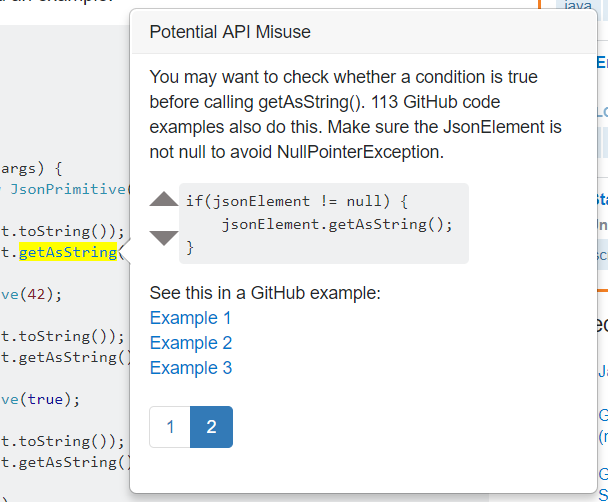
\includegraphics[width=\textwidth, height=6cm]{json_ex3.PNG}
%  \caption{A page describing a way to avoid a {\tt ClassCastException} by checking whether the {\tt JsonElement} object is a primitive.}
%  \label{fig:page2}
%  \end{subfigure}
%  \hfill
%  \vspace{0.02\textwidth}
%\caption{The two pages of a popup generated on {\tt JsonElement.getAsString}.\todo{Can we also show how many users like or dislike the violations in the popup window? Since we don't have any real users, maybe we need to create some artificial numbers for the demonstration purpose.}}
%\label{fig:features}
%\end{figure*}

Suppose Alice needs to read attribute values from a json message using Google's Gson library, which she is not familiar with. Alice finds a Stack Overflow answer post that reads a specific json message posted in the corresponding question post.\footnote{\url{https://stackoverflow.com/questions/29859683/assistance-with-json-from-url}} Though the answer post is accepted as the correct answer, this post does not properly use {\ttt JsonElement.getAsString} (line 7 in the snippet in Figure~\ref{fig:screenshot}), which gets the string value of a json element. For example, if the requested attribute does not exist in the json message, the preceding API call, {\ttt JsonObject.get} (line 2) may return {\ttt null}, which consequently leads to {\ttt NullPointException} when calling {\ttt getAsString} on the returned object. If Alice puts too much trust on this example, she may inadvertently follow a suboptimal solution, which may crash her program in some corner cases. 

Alice can not easily recognize this potential limitation in the given Stack Overflow post. She may have to manually investigate many other posts till finding a code example with ideal API usage. In practice, however, programmers often examine a handful of search results due to the limited time and attention~\cite{brandt2009two, starke2009working, duala2012asking}. {\tool} frees Alice from this manual investigation labor by constrasting a Stack Overflow post with common API usage patterns learned from over 380K GitHub repositories. {\tool} then highlights the API calls that have potential API usage violations in a Stack Overflow post, as shown in Figure~\ref{fig:screenshot}. 

%(1) a check to make sure that the {\tt JsonElement} object is of the type {\tt JsonPrimitive} by using {\tt JsonElement.isJsonPrimitive} before calling {\tt getAsString}, and (2) a check to make sure that the {\tt JsonElement} object is not null before calling {\tt getAsString}. 
{\bf Stack Overflow Popup View.} Alice is interested in learning more about the API and what specifically the code snippet did not include, so she clicks on the highlighted text. Clicking on the highlighted text reveals a popup, as shown in Figure~\ref{fig:screenshot}. The popup is populated with information about any required patterns in {\tool}'s database this particular API call does not adhere to. Alice notices that there are two pages of the popup, indicating two different usage patterns that this call does not follow, as shown in Figure~\ref{fig:page1} and Figure~\ref{fig:page2}. 

\begin{figure}
\centering
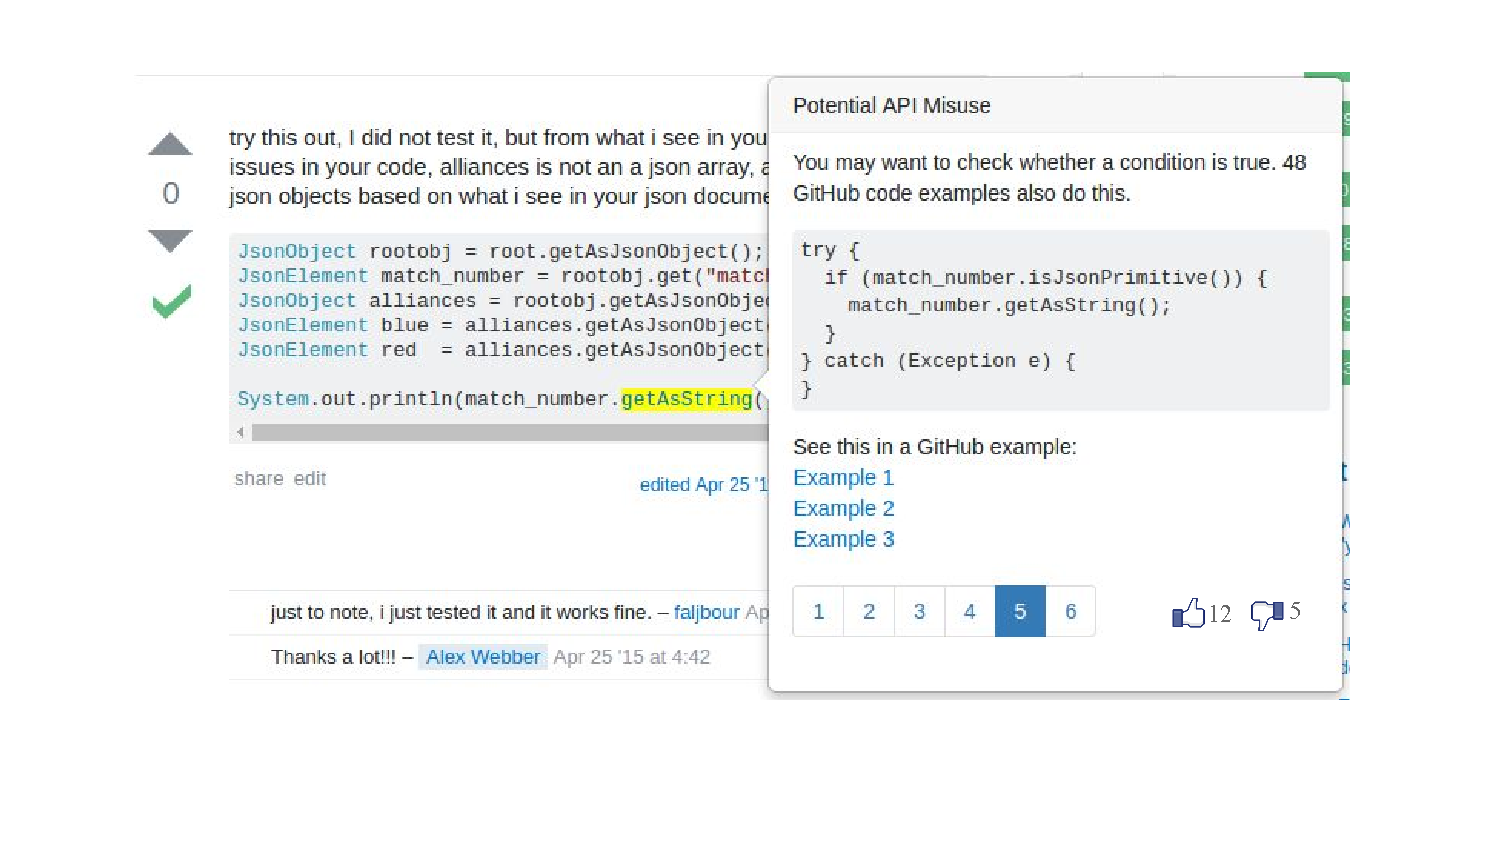
\includegraphics[width=0.5\textwidth]{soap-v2-2.pdf}
  \vspace{.1in}
  \caption{Another API usage warning that reminds programmers to check whether the {\ttt JsonElement} object represents a Json primitive value by calling the {\ttt isJsonPrimitive} method. Otherwise, it may throw  {\ttt ClassCastException}.}
  \label{fig:screenshot2}
\end{figure}

Alice inspects the first page (Figure~\ref{fig:page1}) and sees a warning message, automatically generated by {\soa} for that particular API misuse. She learns that she should check whether the {\tt JsonElement} object is null before calling {\tt getAsString}. She notices that 113 other GitHub code examples use this pattern, which gives her a quantitative measurement of how prevalent this pattern is in real-world projects. Below this is a code example following the required pattern, generated by {\soa} based on the context of the SO example.

Alice then inspects the second page (Figure~\ref{fig:page2}), and finds that it suggests to check whether the {\tt JsonElement} object is primitive before calling {\tt getAsString} to avoid a {\tt ClassCastException}. She notices that this pattern has less than half the support of the previous pattern.

Curious to see the first pattern in context, Alice returns to the first page of the popup and clicks on the first link provided to her under ``See this in a GitHub example.''

%\begin{figure*}[t!]
%\centering
%  \begin{subfigure}[t]{0.48\textwidth}
%  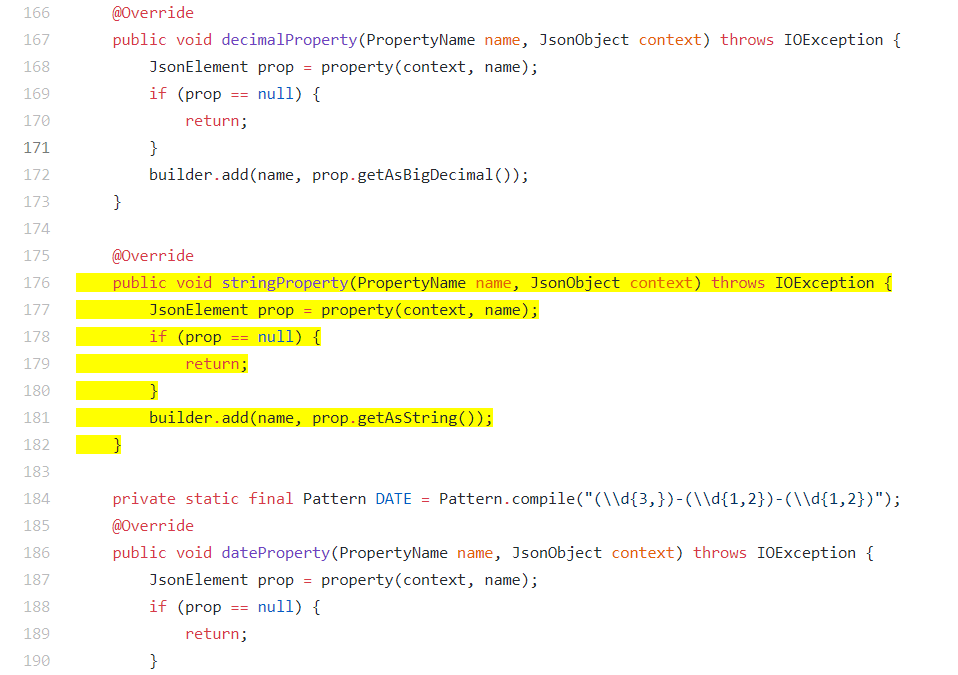
\includegraphics[width=\textwidth]{json_null_gh2_context.PNG}
%  \caption{The second GitHub example for Figure~\ref{fig:page1} in the context of its GitHub file.\protect\footnotemark} 
%  \vspace{.1in}
%  \label{fig:github1}
%  \end{subfigure}
%  \hfill
%  \begin{subfigure}[t]{0.48\textwidth}
%  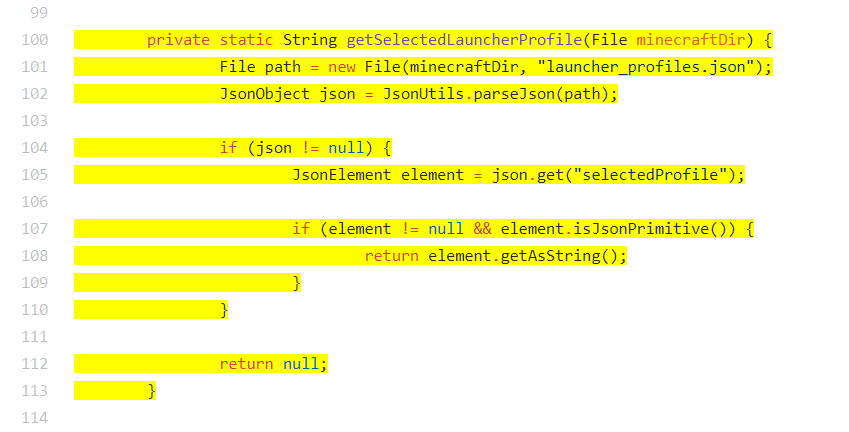
\includegraphics[width=\textwidth]{json_primitive_gh1.PNG}
%  \caption{The first GitHub example for Figure~\ref{fig:page2}.\protect\footnotemark}
%  \vspace{.1in}
%  \label{fig:github2}
%  \end{subfigure}
%  \hfill
%\caption{The GitHub examples redirected to from the links provided in the popup, highlighted by the Chrome extension.\todo{The snapshot only shows the highlighted code. Is there a better way to give paper reviewers some context that the highlighted code is from GitHub and that the code is selectively highlighted by our tool instead of by GitHub?}}
%\label{fig:github_examples}
%\end{figure*}

%\begin{figure}
%\centering
%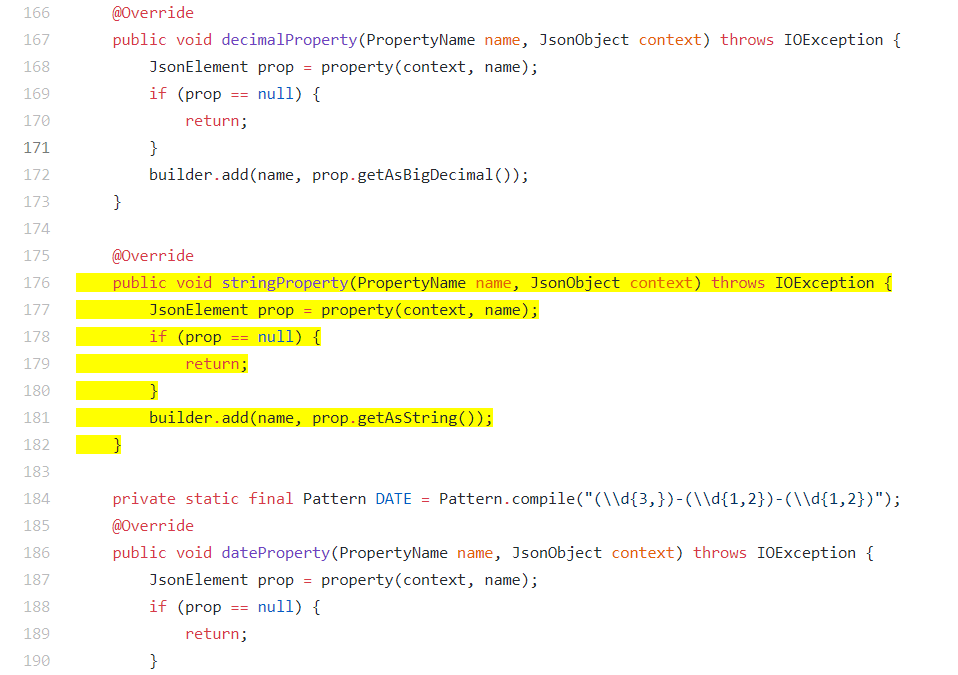
\includegraphics[width=0.48\textwidth]{json_null_gh2_context.PNG}
  %\caption{The GitHub example that a link from Figure~\ref{fig:page1} redirects to, highlighted by the Chrome extension.\protect\footnotemark} 
  %\label{fig:github_examples}
%\end{figure}

{\bf GitHub Example View.} When Alice clicks on one of the GitHub links, the file opens in a new tab and the view scrolls to where the API is called in the file, and the method in which this occurs is highlighted so Alice can easily find it, as seen in Figure~\ref{fig:github_examples}. The addition of a compilable code example that demonstrates the pattern in context can aid Alice in understanding how to use the pattern if it is unfamiliar to her. In this case, Alice finds herself redirected to the method in a GitHub project seen in Figure~\ref{fig:github_examples}.

Returning to the popup in Stack Overflow, Alice clicks on the second link provided for the second page to compare usage patterns in context. This link opens up to the GitHub method seen in Figure~\ref{fig:github2}. She notices that the example uses a null check in conjunction with the primitive check, which makes sense to her after seeing that both were missing from the Stack Overflow code snippet. However, she notes that the more commonly-used pattern only uses a null check.

After seeing these two examples, Alice can infer that a null check is more necessary and is more common than the primitive check, based on the GitHub examples she has seen as well as the GitHub support indicated by the popup message. She upvotes the null check's pattern by clicking on the up-arrow on its page (see Figure~\ref{fig:page2}) to send the server her feedback on the patterns it gave her.

\begin{figure}
\centering
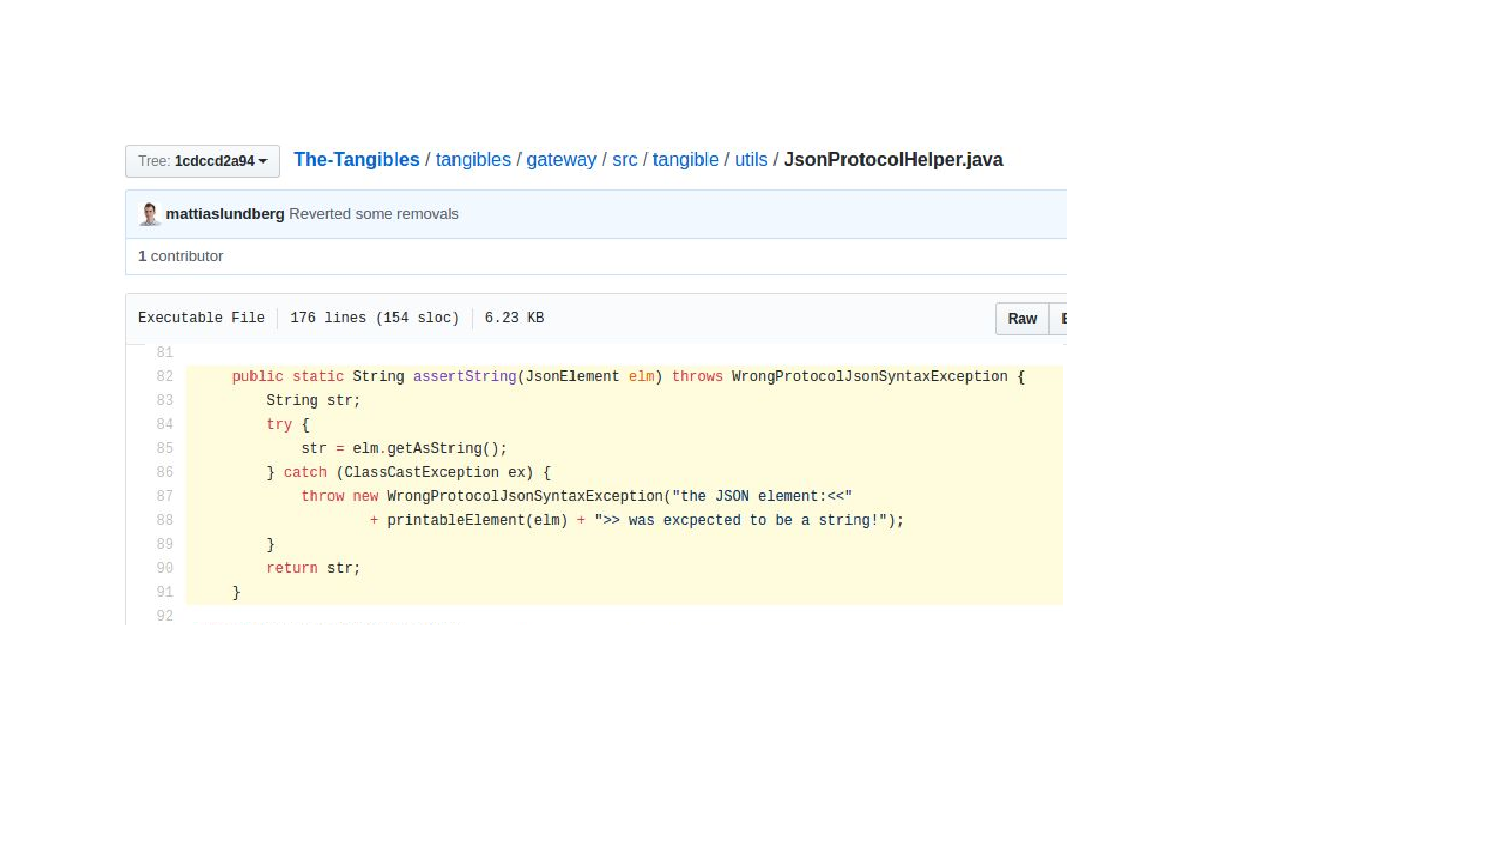
\includegraphics[width=0.5\textwidth]{github-example.pdf}
  \vspace{.1in}
  \caption{{\tool} will redirect the programmer to a highlighted concrete code example in GitHub that follows the correct API usage pattern, when she clicks on one of the three GitHub example links in the pop-up window.\protect\footnotemark}
  \label{fig:github}
\end{figure}

\footnotetext{\url{https://goo.gl/dV4wTh}}

%https://github.com/asakusafw/asakusafw/blob/cad94753128bd3168e23c0539cc55c7e5a653dbd/asakusa-test-data-provider/src/main/java/com/asakusafw/testdriver/json/JsonObjectDriver.java
%\footnotetext{http://tinyurl.com/JsonObjectDriver}

%https://github.com/Spoutcraft/Spoutcraft/blob/5cbbc2b07edaf4194a36130a7e74321e5b30ace0/src/main/java/com/prupe/mcpatcher/Config.java
%\footnotetext{http://tinyurl.com/SpoutcraftConfig}